%Copyright 2019 Christopher M. Jermaine (cmj4@rice.edu) and Risa B. Myers (rbm2@rice.edu)
%
%Licensed under the Apache License, Version 2.0 (the "License");
%you may not use this file except in compliance with the License.
%You may obtain a copy of the License at
%
%    https://www.apache.org/licenses/LICENSE-2.0
%
%Unless required by applicable law or agreed to in writing, software
%distributed under the License is distributed on an "AS IS" BASIS,
%WITHOUT WARRANTIES OR CONDITIONS OF ANY KIND, either express or implied.
%See the License for the specific language governing permissions and
%limitations under the License.
%===============================================================
\documentclass[11pt]{article}

\usepackage{fullpage}
\usepackage{times}
\usepackage{url}
\usepackage[normalem]{ulem}
\usepackage{epsfig} 

\usepackage{subfigure}
\usepackage{graphicx}
\usepackage{titlesec}
\usepackage{multirow}

\titlespacing{\section}{0pt}{3mm}{1mm}
\titlespacing{\subsection}{0pt}{2mm}{0.5mm}
\titlespacing{\subsubsection}{0pt}{2mm}{0.8mm}

\newcommand{\muhat}{\hat{\mu}}
\newcommand{\sigmahat}{\hat{\sigma}}
\newcommand{\todo}[1]{[\textbf{TODO: #1}]}
\newcommand{\eat}[1]{} % TO MAKE LARGE BLOCKS OF TEXT INVISIBLE
\newcommand{\sz}[1]{\lvert#1\rvert}
\newcommand{\card}[1]{\lvert#1\rvert}
\newcommand{\xp}[2]{P \if*#1\else^{#1}\fi \if*#2\else_{\! #2}\fi}
\newcommand{\pr}[3]{\xp{#1}{#2}\left\{\,#3\,\right\}}
\newcommand{\prl}[3]{\xp{#1}{#2}\{\,#3\,\}}
\renewcommand\:{\colon} % for use with \sset, etc.
\newcommand{\sset}[1]{\left\{\,#1\,\right\}}
\newcommand\xD{\mathcal{D}}
\newcommand\xP{\mathcal{P}}
\newcommand\xS{\mathcal{S}}
\newcommand\xbar{\bar x}
\newcommand\vbar{\bar v}
\newcommand\xmax{{x_{\text{max}}}}
\newcommand\eps{\epsilon}
\newcommand{\eeblk}{\hbox{\lower 1pt \vbox{\hrule width6pt\hbox to
  6pt{\vrule height5pt depth1pt \hfil\vrule height5pt depth1pt} \hrule
  width6pt} \unskip}}
\newcommand{\eblk}{{\unskip\nobreak\hfil\penalty50
  \hskip1em\hbox{}\nobreak\hfil\eeblk
  \parfillskip=0pt\finalhyphendemerits=0\par}}
\newtheorem{xample}{Example}
%\newenvironment{example}{\begin{xample}\em}{\eblk\end{xample}}
\makeatletter
\newenvironment{sql}%
 {\vskip 5pt\begin{list}{}{%
  \setlength{\topsep}{0pt}\setlength{\partopsep}{0pt}\setlength{\parskip}{0pt}%
  \setlength{\parsep}{0pt}\setlength{\labelwidth}{0pt}%
  \setlength{\rightmargin}{0pt}\setlength{\leftmargin}{0pt}%
  \setlength{\labelsep}{0pt}%
  \obeylines\@vobeyspaces\normalfont\ttfamily%
  \item[]}}
 {\end{list}\vskip5pt\noindent}
\makeatother
\newcommand{\bpar}[1]{\vskip 5pt\noindent\textbf{#1}\hskip 1em}
\newcommand\yN{{\tilde N}}
\newcommand\yX{{\tilde X}}
\newcommand\ymu{{\tilde\mu}}
\newcommand\ysigma{{\tilde\sigma}}


\newcommand{\goodgap}{
        \hspace{\subfigtopskip}
        \hspace{\subfigbottomskip}
}

%\renewcommand{\baselinestretch}{0.99}

\newtheorem{definition}{Definition}
\newtheorem{Rule}{Rule}
\newtheorem{lemma}{Lemma}
\newtheorem{theorem}{Theorem}
\newtheorem{problem}{Problem}
\newtheorem{example}{Example}
\newtheorem{optimization}{Optimization}
\newtheorem{observation}{Observation}
\newtheorem{corollary}{Corollary}

\newcommand{\qed}{\hspace*{\fill}
           \vbox{\hrule\hbox{\vrule\squarebox{.667em}\vrule}\hrule}\smallskip}

\long\def \ignoreme#1{}

\def\qed{\hfill \mbox{\rule[0pt]{1.5ex}{1.5ex}}}



\begin{document}
%\maketitle
%\pagestyle{empty}

\begin{center}
{\bf \huge{Data Science Tools and Models: Deep Learning with TensorFlow}}
\end{center}


\section{Description}

In this assignment, you will be using Google's open-source TensorFlow machine learning tool to implement
some deep learning architectures that will be used to classify sequences of raw text (This time, no
pre-processing using dictionaries and words. We will be operating on raw characters!). Since deep learning
is computationally expensive, it is strongly recommended that you use one of Amazon's deep learning machines
to do this assignment (see below). The small learning problems we'll consider will take about 10-20
minutes max using one of these machines, but might take 10 times as long (or more) using a laptop. Plus,
TensorFlow can be a bit of a pain to install on your laptop, so using Amazon or Google Colab is just plain easier. The only
situation in which you might consider using your own hardware is if you've got a tricked out laptop/desktop
with a beefy GPU for game playing that TensorFlow can make use of.

In this assignment, you will be classifying 80 character chunks of journal titles.

\section{WorkingWith a Partner}
For this assignment, unlike previous assignments, you are welcome to work with a partner. You don't
have to work with a partner; the assignment is doable without one. We estimate 15 hours of work for an
average student to complete all three tasks.
If you do work with a partner, make sure to put \textbf{both} partner's names in the write-up you submit.
And only \textbf{one} partner should turn in the assignment.


\section{AWS or Google Colab (review of Lab 7)}
This assignment may be completed on either AWS or Google Colab. Please refer to the appropriate section for starting points.

\subsection{Running TensorFlow on AWS }

To get started, log on to Amazon AWS, then click on ``EC2'', and ``Launch Instance''. You will be asked
for a machine instance to start up (this will govern the software on the machine you run). Scroll down to
``Deep Learning AMI (Ubuntu)'' and click ``Select''. This machine instance (not
surprisingly, given the name) has a number of deep learning tools installed on it. Next you need to choose
the machine type you will rent. You will want to choose a machine with a GPU, which will make your deep
learning codes much faster. Choose ``p2.xlarge'' and ``Review and Launch''. You want to make sure that you
can SSH into your machine, so choose ``Edit Security Groups'' then click ``Add Rule'' to make sure to allow
SSH access from Anywhere. Once you have done that, click ``Review and Launch'' and then ``Launch''. You can find your
machine by going to the EC2 Dashboard and then clicking on ``Running Instances''.

As usual, when you are done with your machine, \textbf{MAKE SURE TO SHUT IT DOWN!!}

\subsection{What to Turn in}
Turn in a text document (or PDF) giving your results for each task, and separately turn in the Python code that you wrote. DO NOT put Python code in a PDF.

\subsection{Running TensorFlow on Google Colab }

You may complete this assignment using Google Colab. Please note that we cannot guarantee availability of Colab, so please allow enough time to complete the assignment on AWS, if, for some reason, Colab is not available.

If you use Google Colab, you will need to create a new Colab notebook that contains your code and results. You may modify the Colab notebook from Lab 7, if you like.

\subsection{What to Turn in}
Submit  your new Colab notebook (.ipynb file with all 3 tasks and outputs). 

\section{The Tasks}
There are three separate tasks that you need to complete to finish the assignment.


\subsection{Task 1: (55 points) Adding ``Time Warping'' to the RNN}
Since the lines of text consist of up to 80 characters or so, as discussed in class, unrolling the RNN to
perform learning means that we have to backdrop through up to 80 layers. Thus, the ``vanishing gradient''
problem will be very real. The result is that after 10,000 training iterations, the learned RNN is only able to
average around 50-60 correctly classified lines in each training batch. Running for more iterations (past the
original 10,000) is not going to be very helpful.

Given this, the next thing that we'll do is to use a (non-standard) trick to make the learner perform a bit
better. What we'll do is to change the NN architecture slightly so that it implements ``time warping''. That
is, rather than the state of the network being fed-forward not only to the next time tick, you'll change the
network so that the state is also fed forward ten time ticks into the future. This means that it will be possible
to backpropagate through 80 time ticks in only 8 hops, and so vanishing gradients will be much less problematic.

To do this, you will want to modify that your weight matrix for moving from state-to-state so that it is
(256 + \texttt{hiddenUnits} + \texttt{hiddenUnits}) by (\texttt{hiddenUnits}) matrix. The first 256 values encode the
character at the current time tick, the next set of input values are the state from the last time tick, and the last
set of input values is the state from ten time ticks ago. The reason we call this ``time-warping'' is that we are
feeding the state at time tick $i$ to time-tick $i$ + 10. That's the time warp.

A visualization of the time warp, with a distance of 3, is shown in the figure below.

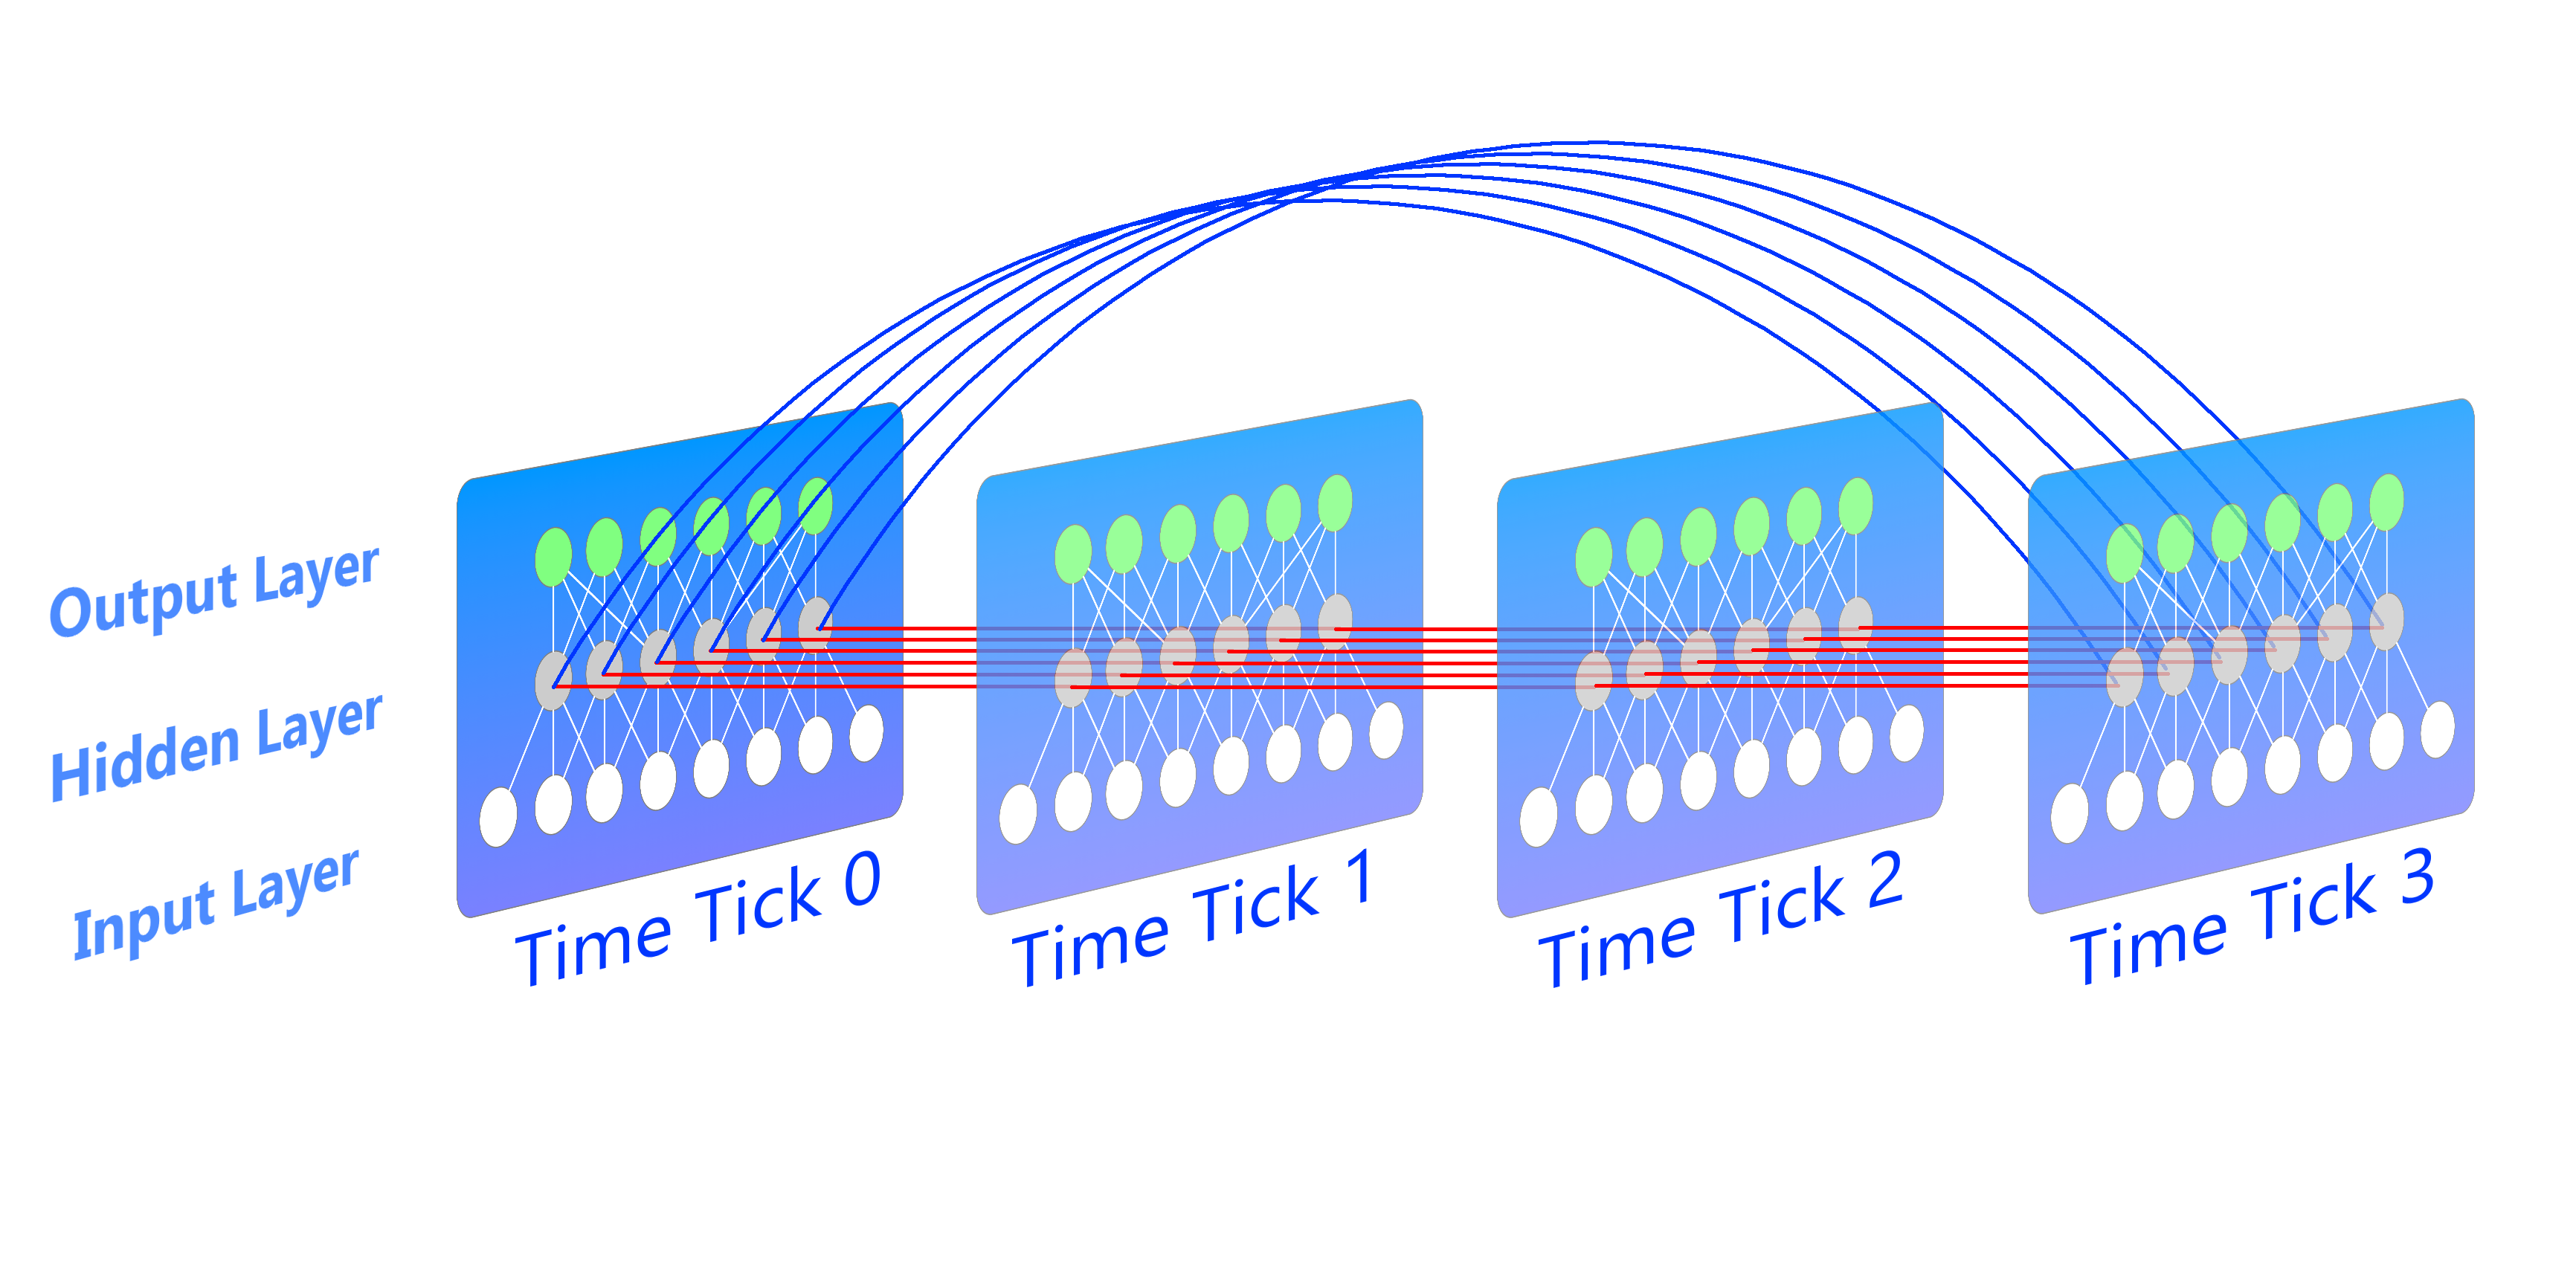
\includegraphics[width=0.6\textwidth]{RNN_diagram.png}

Note that to implement the time warping, you need to have some data structure that saves the state
vectors as they are produced. Then, ten time ticks later this saved state will be used. For the first ten time
ticks (where it is not possible to take the state from 10 time ticks ago as input) you'll take as input a special
vector of values whose optimal values should be learned (this, make this special vector a \texttt{tf.Variable}).

The whole point of TensorFlow is that you can (in a few lines of code) change how information flows
through the network, and the system will automatically differentiate the resulting network and figure out
how to learn it. That is cool!

Since the time-warping will double the number of activations that are pushed through the weight matrix,
you should go ahead and halve the size of the hidden state to compensate. That is, rather than having the
hidden state be 1,000 activations, you should make it consist of 500 activations.

Once you have made these modifications, run the resulting code for the full 10,000 iterations, and copy
and paste the output for the last 20 iterations, plus the final average loss from the last 10 mini-batches, into your turn in document. 

Note that our line of text representation is a matrix (a sequence of vectors, where each vector was a one-hot encoding of a character) as shown below:

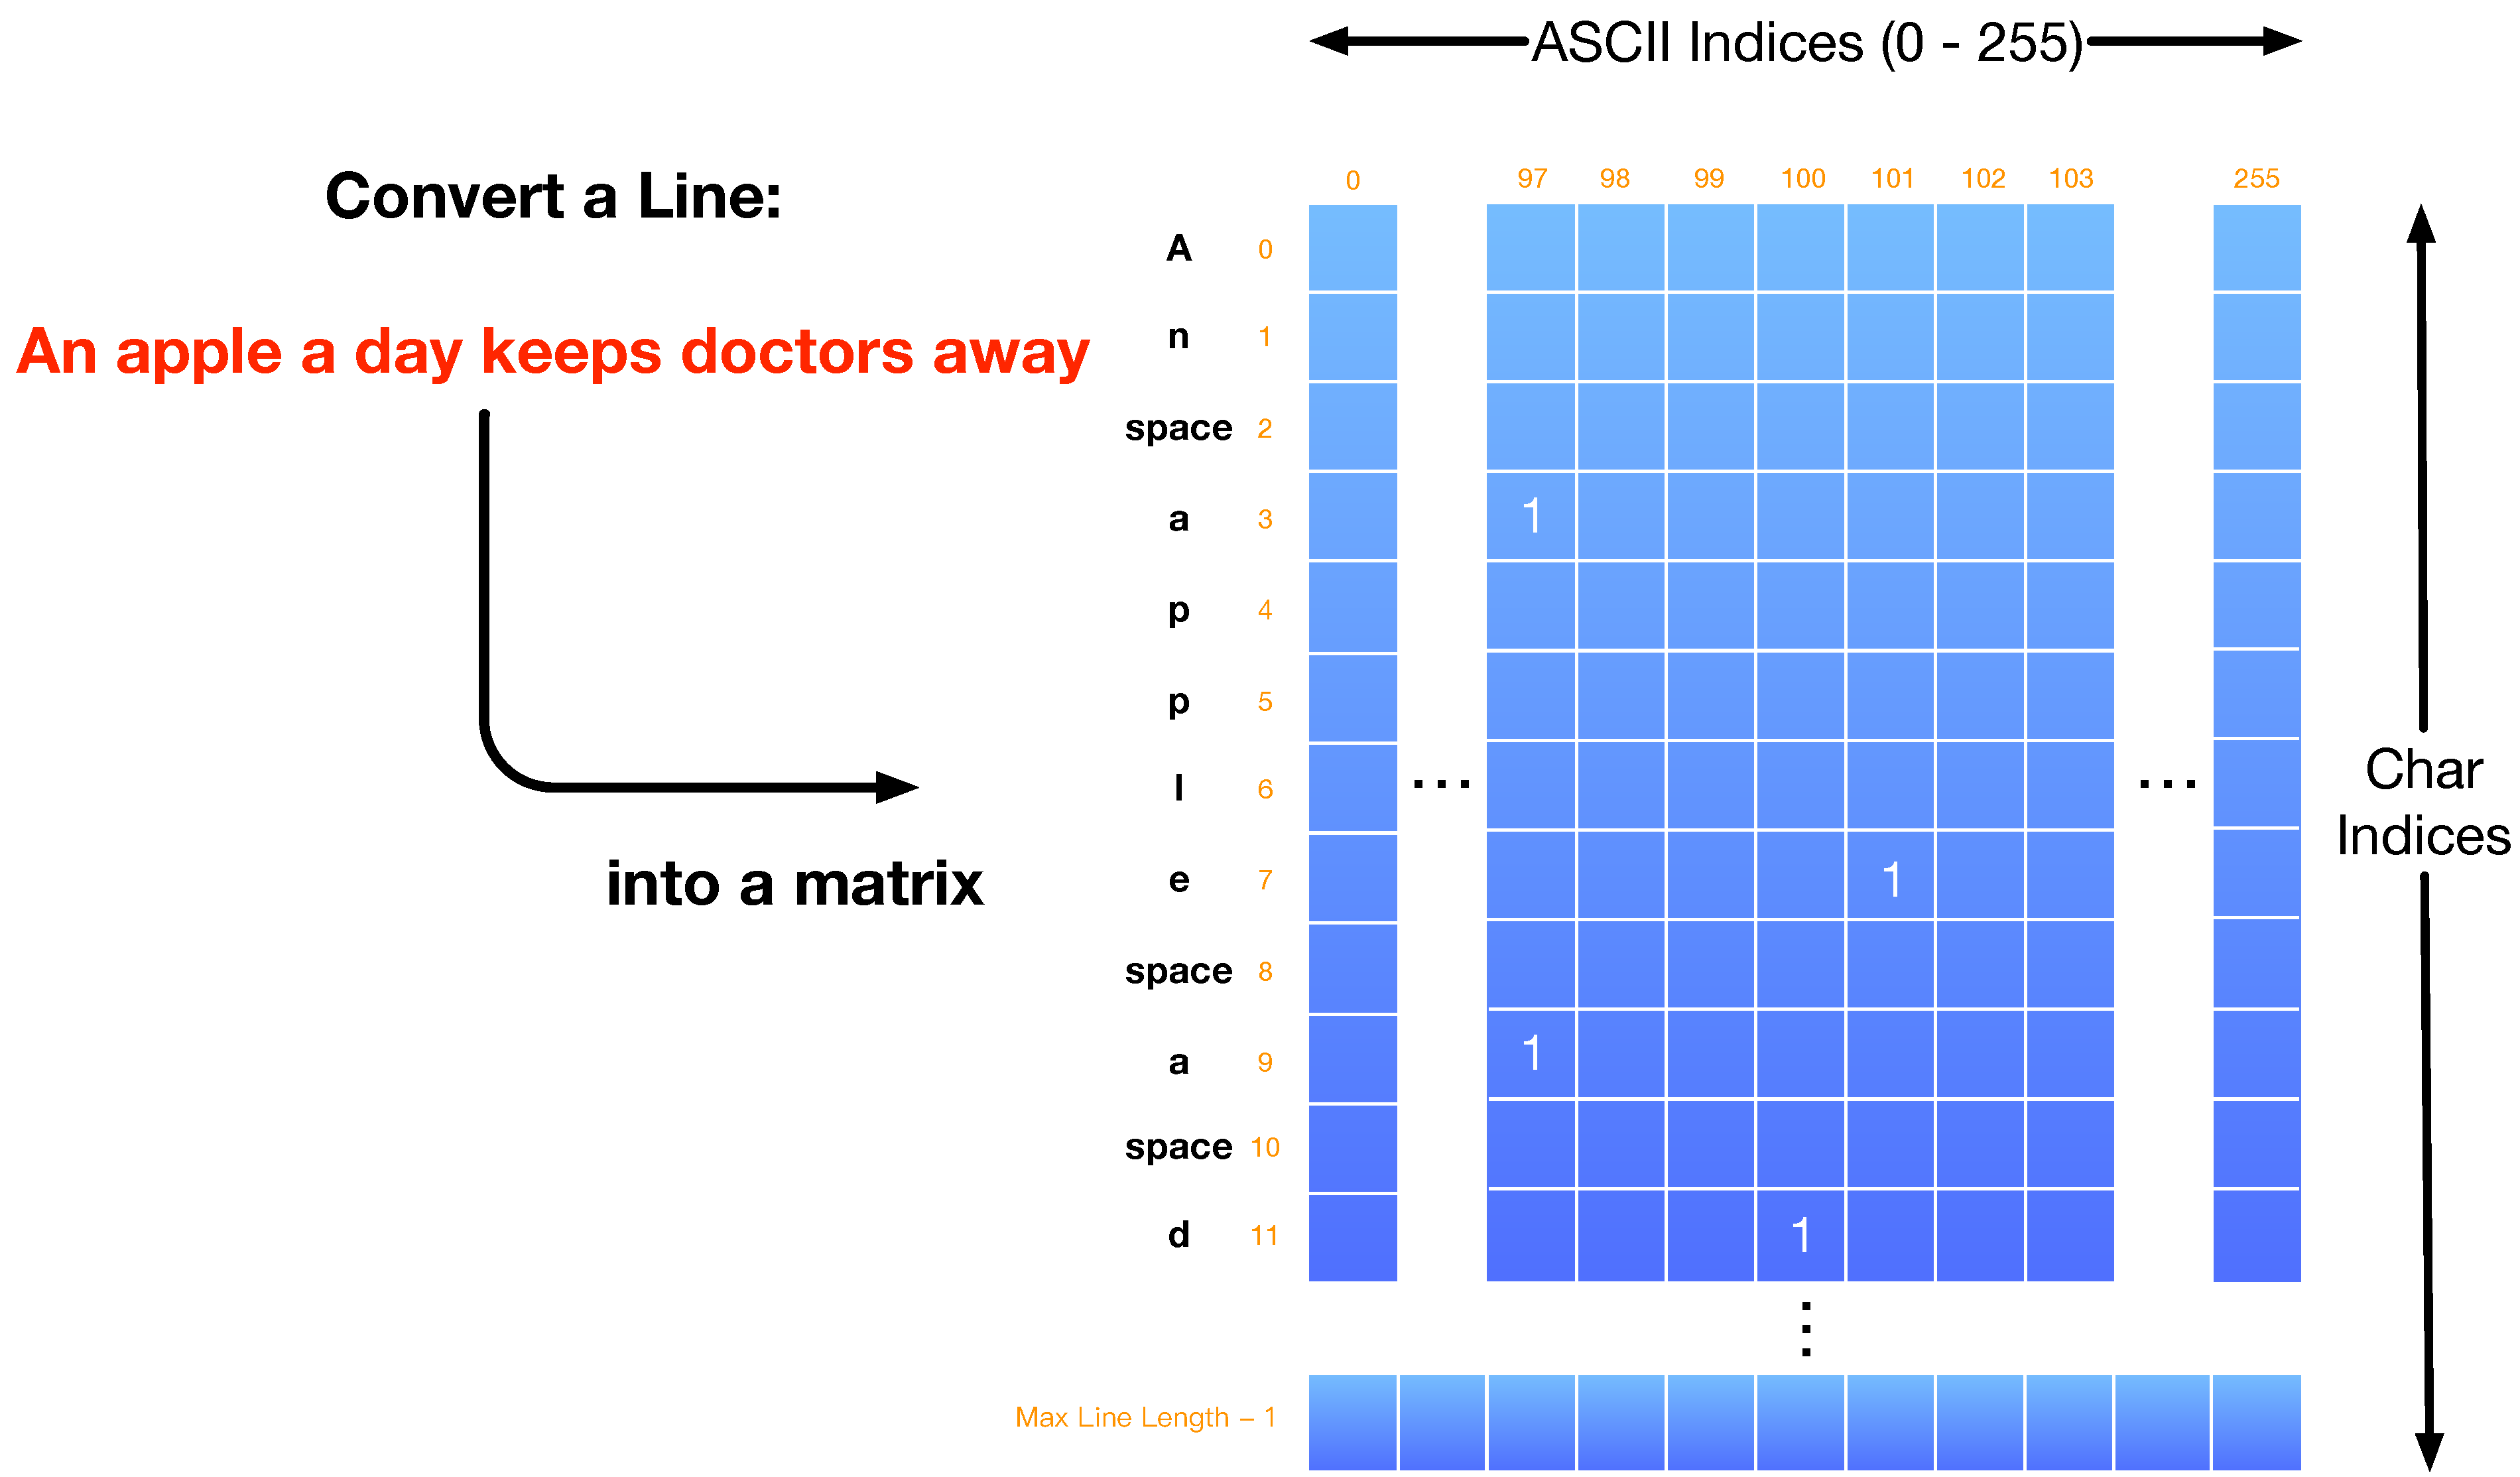
\includegraphics[width=0.6\textwidth]{onehotencoding.pdf}

A visual representation of the batch is:

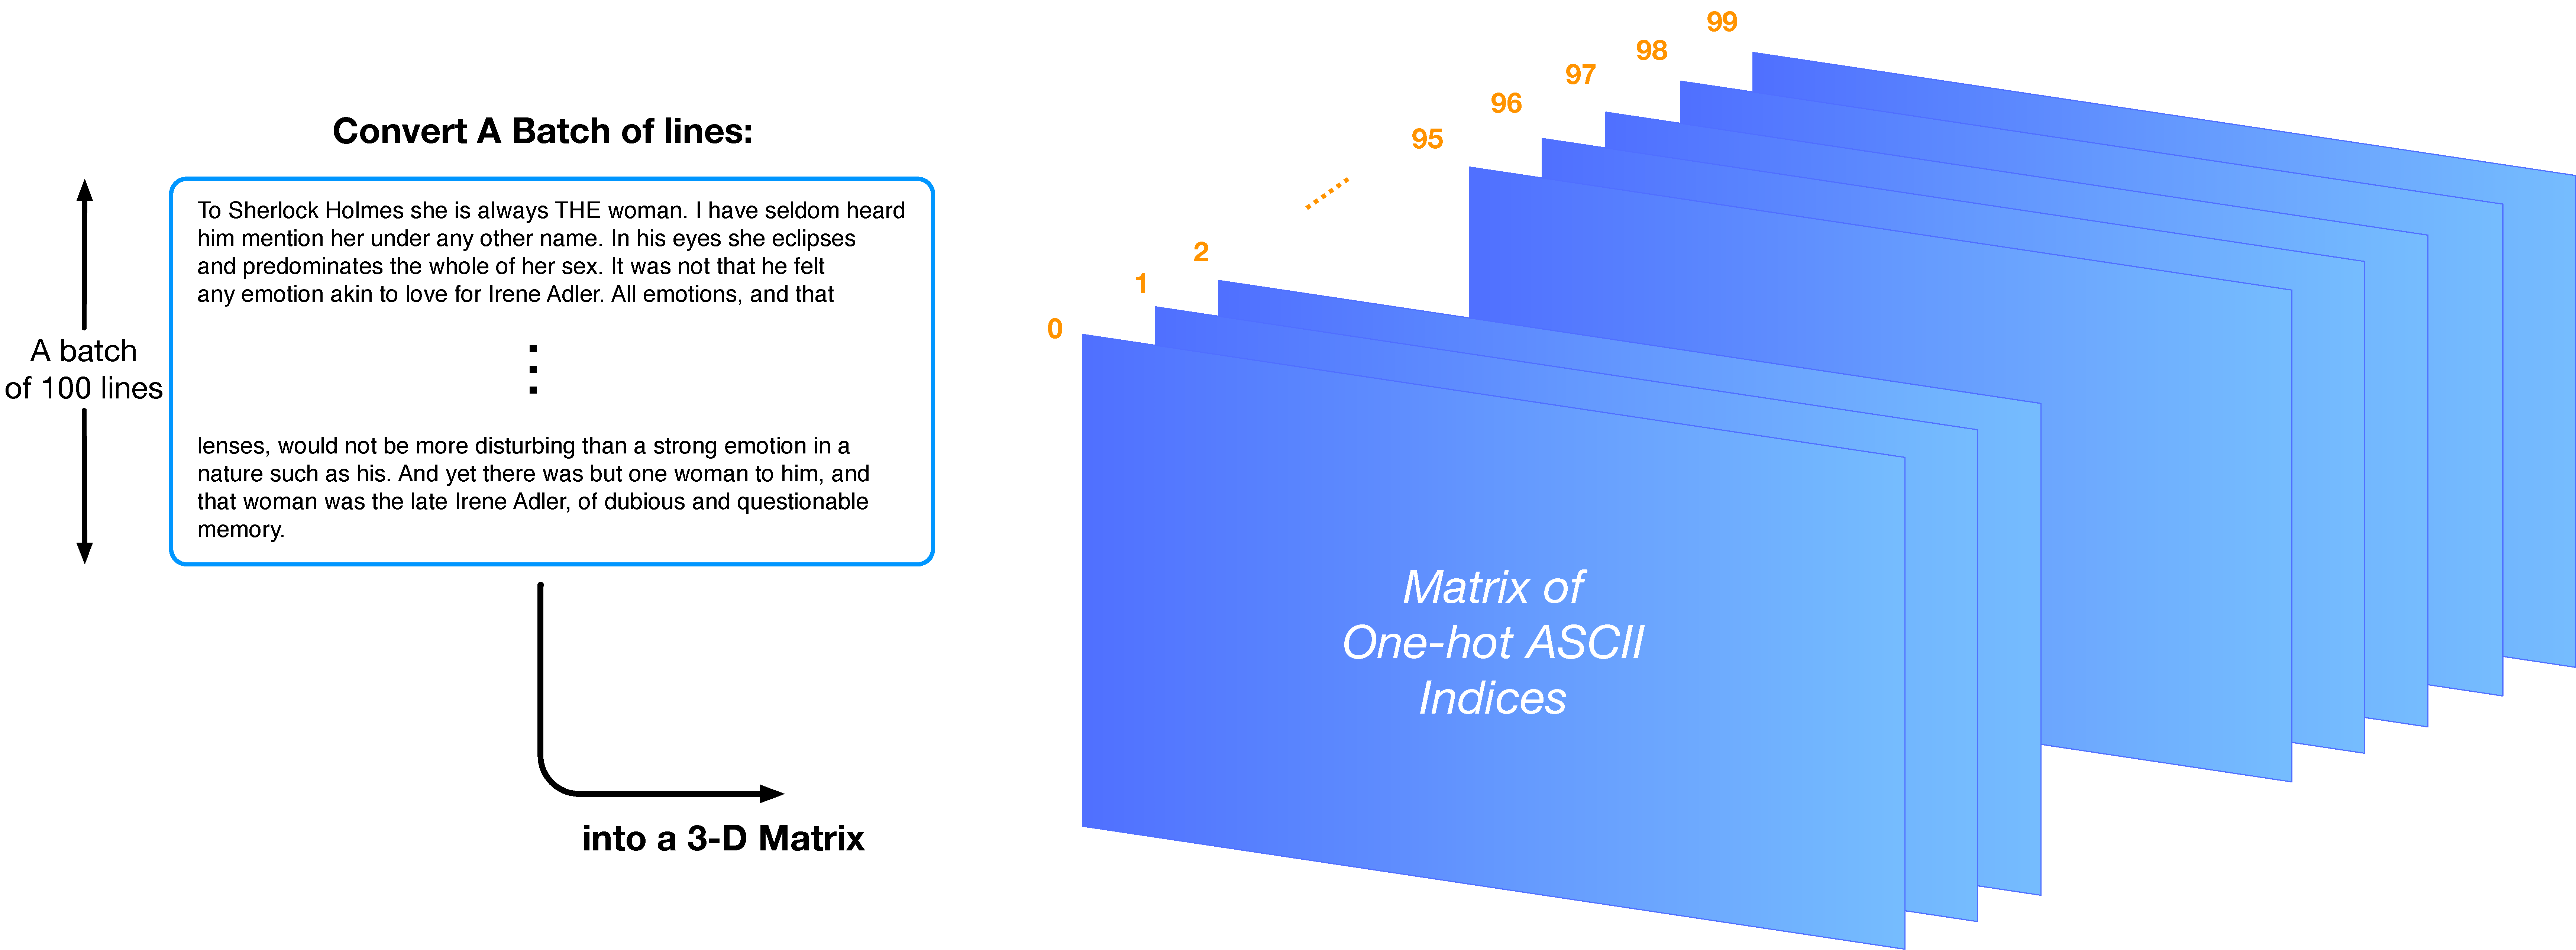
\includegraphics[width=0.6\textwidth]{batch.pdf}


\subsection{Task 2: (40 points) Implementing a Feed-Forward Network} 
That's all you have to do to get a C on the assignment. Now, to get up into A territory, the next modification
that you will make is more substantial. Now you will change the code so that it no longer implements
an RNN, but instead it implements a simple feed-forward network with one hidden layer. For the RNN, our
line of text representation was a matrix. Now, our text representation will be a single vector, where each vector has all of the vectors
encoding each of the characters, appended end-on-end. Note that I've already supplied you with a function
that supplies mini-batches of data in this format, so you can just use my function to create batches of training
data for learning. All you need to do is to figure out how to modify the network to make use of this function.

Once you have made these modifications, again run the resulting code for the full 10,000 iterations, and
copy and paste the output for the last 20 iterations, plus the message that you added, into your turn in document.


You can't possibly use the learned network to classify a sequence
that is longer than the width of the input layer that you trained. The RNN, in contrast, could be used to
classify an input sequence of any length.

\subsection{Task 3: (5 points) Implementing an LSTM Network}
Here, you will modify the RNN implementation so that it makes use of TensorFlow's built-in
LSTM modules. A bit of web-surfing will give you plenty of examples of how to use them. Again, run
the resulting ode for 10,000 iterations, and copy and past the output into your turnin.

\section{Getting Better Results}
Once you have your networks working, try to get better results!

Some things you can play with include:
\begin{itemize}
\item Learning rate % best for task 2 at 0.1
\item Optimizer used
\item Batch size
\item Hidden unit size % better at 128
\end{itemize}

Note that larger values do not always produce better results.\\

Following the tasks as described above, we got ~48\% correct labeling for Task 1, ~55\% for Task 2, and ~50\% for Task 3. With some minor adjustments, we were able to get 97\% accuracy for Task 2. 


\end{document}
